\documentclass[12pt,a4paper]{article}

\usepackage[utf8]{inputenc}
\usepackage[T5]{fontenc}
\usepackage[vietnamese,english]{babel}
\usepackage{mathptmx}
\usepackage[a4paper,margin=1.95cm]{geometry}
\usepackage{array}
\usepackage{amsmath}
\usepackage{booktabs}
\usepackage{enumitem}
\usepackage{float}
\usepackage{graphicx}
\usepackage{longtable}
\usepackage{subcaption}
\usepackage{tabularx}
\usepackage{tikz}
\usepackage{xcolor}
\usepackage[unicode]{hyperref}
\usetikzlibrary{arrows.meta,positioning}

\graphicspath{{assets/}}

\hypersetup{
  colorlinks=true,
  linkcolor=black,
  urlcolor=blue
}

\setlength{\parindent}{0pt}
\setlength{\parskip}{4pt}
\setlist[itemize]{leftmargin=1.05cm,itemsep=2pt}
\setlist[enumerate]{leftmargin=1.05cm,itemsep=2pt}
\renewcommand{\arraystretch}{1.12}

\newcolumntype{Y}{>{\raggedright\arraybackslash}X}
\newcolumntype{P}[1]{>{\raggedright\arraybackslash}p{#1}}
\definecolor{Ink}{HTML}{1F2933}

\begin{document}

\begin{titlepage}
\begin{center}

\textsc{\large \textcolor{black}{\textbf{HANOI UNIVERSITY OF SCIENCE AND TECHNOLOGY}}}\\[0.5cm]

{\Large \uppercase{School of Information and Communication Technology}\\[1cm]}


\includegraphics[scale=0.13]{logo-soict-hust-1.png}\\[1cm]
\textsc{\Large \textbf{Parallel and Distributed Programming Report:}}\\[0.4cm]

\rule{\linewidth}{0.7mm} \\[0.4cm]
{\huge \bfseries\color{Ink} MPI Sinkhorn Optimal Transport Solver \\[0.25cm]}
{\Large \bfseries\color{black!70!black} Row-wise Data Decomposition on a Physical VM Cluster \\[0.35cm]}
\rule{\linewidth}{0.7mm} \\[0.9cm]

\color{black!80!black}{\large \textbf{\textit{Course}:}}\\[0.4cm]
\begin{tabular}{l}
\large IT4130E -- Parallel and Distributed Programming \\[0.7cm]
\end{tabular}

\color{black!80!black}{\large \textbf{\textit{Presented by}:}}\\[0.6cm]
\color{black}
\begin{tabular}{l}
\large Nguyễn Tất Thanh - 20235560 \\[0.35cm]
\large Đặng Thịnh Tường Minh - 20235528 \\[0.35cm]
\large Nguyễn Ngọc Minh - 20235533 \\[0.35cm]
\large Kiều Sơn Tùng - 20235571 \\[0.35cm]
\end{tabular}

\vfill

{\large \color{black!80!black}{\textbf{Hanoi - Vietnam}}\\[0.2cm] \color{blue!90!black}2026}

\end{center}
\end{titlepage}
\setcounter{page}{2}

\begin{center}
\textit{This report presents the design, implementation, cluster setup, and benchmark analysis of a C++/MPI Sinkhorn-Knopp solver for entropy-regularized optimal transport on a physical-machine Ubuntu VM cluster.}
\end{center}

\tableofcontents
\newpage

\section{Project Objective and Requirement Coverage}

The course task requires a group of four students to build a real MPI program in C/C++, run it on at least three physical machines, and analyze its parallel behavior. The selected problem is entropy-regularized optimal transport solved by the Sinkhorn-Knopp algorithm. This is a non-trivial dense numerical workload because each iteration performs matrix-vector style computation over an $N \times N$ kernel matrix and must synchronize a global column vector.

\begin{table}[H]
\centering
\begin{tabularx}{\linewidth}{P{4.2cm}Y}
\toprule
\textbf{Requirement from task file} & \textbf{How this project satisfies it} \\
\midrule
At least three physical machines & Benchmarks were run on three-machine router/Ethernet and three-machine Wi-Fi clusters; earlier Wi-Fi runs also include a four-machine cluster. \\
C/C++ implementation & The main solver is implemented in \texttt{mpi-sinkhorn-step/cpp/sinkhorn\_cpp.cpp}. \\
Demoable MPI program & The executable supports \texttt{--mode sequential} and \texttt{--mode mpi}; MPI runs use OpenMPI hostfiles and SSH. \\
Parallelism type and decomposition & Data-level parallelism with one-dimensional row-wise data decomposition. \\
Mapping and communication strategy & Rows are mapped to ranks; each iteration uses local dense compute and \texttt{MPI\_Allreduce} for the global column update. \\
Load-balance analysis & Per-rank compute and communication times are exported to JSON and summarized in the report. \\
Correctness validation & MPI objective/error metrics are compared against sequential output with the same random seed and iteration count. \\
Runtime, speedup, efficiency & The report includes size sweep, process sweep, workload calibration, $2N$ speedup, router-vs-Wi-Fi, and dynamic scheduling experiments. \\
\bottomrule
\end{tabularx}
\caption{Mapping from assignment requirements to project deliverables.}
\end{table}

\subsection{Team Work Allocation}

\begin{table}[H]
\centering
\begin{tabularx}{\linewidth}{P{4.6cm}P{3cm}Y}
\toprule
\textbf{Member} & \textbf{Student ID} & \textbf{Assigned work} \\
\midrule
Nguyễn Tất Thanh & 20235560 & Cluster setup, SSH/OpenMPI configuration, router evidence collection \\
Đặng Thịnh Tường Minh & 20235528 & Sequential baseline, correctness validation, Python vs C++ comparison \\
Nguyễn Ngọc Minh & 20235533 & Load-balance analysis, compute/communication metrics, result visualization \\
Kiều Sơn Tùng & 20235571 & MPI implementation, row-wise decomposition, benchmark run scripts \\
\bottomrule
\end{tabularx}
\caption{Team work allocation for implementation, experiments, and result analysis.}
\end{table}

\section{Problem and Sequential Algorithm}

Optimal transport searches for a transport matrix $P$ that moves a source distribution $a$ to a target distribution $b$ while minimizing a cost matrix $C$. The entropy-regularized version adds a smoothing term and can be solved efficiently by Sinkhorn-Knopp iterations. Given $\varepsilon > 0$, define the kernel
\[
K_{ij} = \exp(-C_{ij}/\varepsilon).
\]
The solver alternates between two scaling vectors:
\[
u = a \oslash (K v), \qquad
v = b \oslash (K^T u).
\]
The final transport plan is implicitly represented as
\[
P = \mathrm{diag}(u)K\mathrm{diag}(v).
\]

The sequential algorithm stores the full dense kernel matrix and performs the following work in each iteration:

\begin{enumerate}
  \item Compute every denominator $(Kv)_i$ and update $u_i$.
  \item Compute every denominator $(K^Tu)_j$ and update $v_j$.
  \item Optionally compute row error, column error, and transport objective for validation.
\end{enumerate}

For an $N \times N$ dense matrix, the main computational cost is $O(N^2)$ per iteration and memory usage is also $O(N^2)$. This explains why larger sizes provide more parallel work but also stress VM memory.

\section{Parallel Algorithm Design}

\subsection{Parallelism Type}

The implementation uses \textbf{data-level parallelism}. The matrix is decomposed by rows. Rank $r$ owns a contiguous interval $[s_r,e_r)$:
\[
\mathrm{local\_rows}_r = e_r - s_r.
\]
Every rank stores only its local kernel block $K_r$. The vector $v$ is replicated on all ranks. Rank $r$ can update its local entries of $u$ independently:
\[
u_i = a_i / \sum_j K_{ij}v_j, \qquad i \in [s_r,e_r).
\]

\subsection{Communication and Topology}

After updating local $u$, each rank computes a partial column contribution:
\[
\mathrm{local\_col}_j = \sum_{i=s_r}^{e_r-1} K_{ij}u_i.
\]
The global column denominator is obtained with
\[
\mathrm{global\_col} = \mathrm{MPI\_Allreduce\_sum}(\mathrm{local\_col}).
\]
Then every rank can update the replicated vector $v$:
\[
v_j = b_j / \mathrm{global\_col}_j.
\]

The logical communication pattern is collective rather than master-worker. In practice, OpenMPI chooses an internal reduction algorithm depending on process count and network. The important property for this project is that one length-$N$ vector is reduced in every Sinkhorn iteration. With double precision, the main payload is approximately $8N$ bytes per rank per column synchronization.

\begin{figure}[H]
\centering
\resizebox{0.98\linewidth}{!}{%
\begin{tikzpicture}[
  node distance=0.55cm and 0.65cm,
  block/.style={draw=blue!55!black, fill=blue!6, rounded corners=2pt, align=center, font=\small, text width=2.95cm, minimum height=0.85cm},
  comm/.style={draw=red!55!black, fill=red!6, rounded corners=2pt, align=center, font=\small, text width=2.65cm, minimum height=0.85cm},
  arr/.style={-{Stealth[length=2.2mm]}, thick, draw=black!65}
]
\node[block] (own) {Rank $r$ owns\\ rows $[s_r,e_r)$\\ and local $K_r$};
\node[block, right=of own] (u) {Update local\\ $u_i = a_i / (K_rv)_i$};
\node[block, right=of u] (col) {Accumulate\\ partial column\\ $\mathrm{local\_col}_r$};
\node[comm, right=of col] (red) {\texttt{MPI\_Allreduce}\\ sum length-$N$ vector};
\node[block, right=of red] (v) {Update replicated\\ $v_j=b_j/\mathrm{global\_col}_j$};
\node[block, below=0.7cm of col, text width=4.8cm] (metrics) {Per-rank JSON metrics: local rows, compute time, communication time, objective and marginal errors};
\draw[arr] (own) -- (u);
\draw[arr] (u) -- (col);
\draw[arr] (col) -- (red);
\draw[arr] (red) -- (v);
\draw[arr] (v.south) |- (metrics.east);
\draw[arr] (metrics.west) -| (own.south);
\end{tikzpicture}
}
\caption{C++/MPI Sinkhorn iteration structure. Computation is row-local; the only mandatory synchronization in each iteration is the column-vector \texttt{MPI\_Allreduce}.}
\end{figure}

\subsection{Pseudocode}

\begin{verbatim}
Input: N, epsilon, max_iters, rank r, number of ranks p
Build local row interval [s_r, e_r)
Build local dense kernel K_r
Initialize local u and replicated v

for iter = 1..max_iters:
    for each local row i:
        denom = sum_j K_r[i,j] * v[j]
        u[i] = a[i] / denom

    local_col[:] = 0
    for each local row i:
        for each column j:
            local_col[j] += K_r[i,j] * u[i]

    global_col = MPI_Allreduce_sum(local_col)
    for each column j:
        v[j] = b[j] / global_col[j]

Compute objective/error metrics for validation
Write JSON output with runtime and per-rank metrics
\end{verbatim}

\subsection{Why Row Decomposition Was Chosen}

One-dimensional row decomposition was chosen because it is reliable on a small physical cluster and maps directly to the structure of the Sinkhorn update. A two-dimensional block decomposition could reduce per-rank memory and communication at larger scale, but it would require more complex redistribution of $u$, $v$, and partial sums. For this course project, the row-wise design gives a clear explanation, a robust demo, and measurable speedup.

\section{Implementation}

The C++ implementation is located in \texttt{mpi-sinkhorn-step/cpp/sinkhorn\_cpp.cpp}. The executable accepts command-line options for matrix size, mode, epsilon, seed, maximum iterations, communication mode, partition mode, and output path.

The C++ path is the main deliverable of the project. It uses explicit flat arrays for the local dense kernel block and vectors, so the inner loops are simple contiguous-memory scans. This matters for the benchmark: most useful work is spent in repeated floating-point loops over $K_r$, while the MPI layer only exchanges the column denominator vector. The implementation also emits per-rank timing fields, which makes it possible to separate compute imbalance from communication overhead in later experiments.

\begin{table}[H]
\centering
\begin{tabularx}{\linewidth}{P{4cm}Y}
\toprule
\textbf{Component} & \textbf{Role} \\
\midrule
Sequential solver & Baseline for correctness and speedup. \\
MPI solver & Row partitioning, local dense compute, \texttt{MPI\_Allreduce}, per-rank timing. \\
Benchmark scripts & Run repeated experiments for sizes, process counts, network setups, and partition modes. \\
Summarizers & Convert JSON outputs to CSV/Markdown tables and figures. \\
Dynamic partition modes & Experimental chunk-based scheduling modes for heterogeneous machines. \\
\bottomrule
\end{tabularx}
\caption{Main implementation components.}
\end{table}

Each JSON result contains runtime, objective, row error, column error, hostnames, local rows per rank, rank compute time, rank communication time, and rank total time. These fields are used to compute speedup, efficiency, imbalance, and communication overhead.

\section{Cluster Setup and Router Evidence}


\subsection{Node Hardware and Router Specifications}

The cluster is heterogeneous: the virtual machines expose the same number of virtual CPU cores for the main MPI runs, but the physical processors and memory limits differ. Public CPU scores are included only as a rough reference; actual MPI performance also depends on thermal limits, VM scheduling, memory pressure, and network behavior.

\begin{table}[H]
\centering
\small
\begin{tabularx}{\linewidth}{P{1.4cm}P{2.25cm}P{1.25cm}P{1.15cm}P{1.7cm}P{2.0cm}Y}
\toprule
\textbf{Node} & \textbf{Physical CPU} & \shortstack{\textbf{CPU}\\\textbf{cores /}\\\textbf{threads}} & \shortstack{\textbf{VM}\\\textbf{CPU}} & \shortstack{\textbf{VM RAM}\\\textbf{during}\\\textbf{project}} & \shortstack{\textbf{Geekbench}\\\textbf{6 score}} & \textbf{Role in experiments} \\
\midrule
Master & Intel Core i5-9300H & 4 / 8 & 4 vCPU & 4 GB $\rightarrow$ 8 GB & 1291 single / 3737 multi & Master for router and latest Wi-Fi runs \\
Worker 1 & Intel Core i5-9300H & 4 / 8 & 4 vCPU & 4 GB $\rightarrow$ 8 GB & 1291 single / 3737 multi & Router/Wi-Fi worker \\
Worker 2 & AMD Ryzen 5 5600H & 6 / 12 & 4 vCPU & 3 GB $\rightarrow$ 6 GB & 1594 single / 5716 multi & Router worker, stronger physical CPU but initially memory-limited \\
Worker 3 & Intel Core i3-1115G4 & 2 / 4 & 4 vCPU & 4 GB $\rightarrow$ 6 GB & 1571 single / 3056 multi & Wi-Fi worker used in the latest three-node Wi-Fi run \\
\bottomrule
\end{tabularx}
\caption{Physical machines and VM resource allocation. CPU core/thread counts are from Intel/AMD specifications; Geekbench 6 scores are public user-submitted averages.}
\end{table}

The router used for the wired/router experiment was a TP-Link Archer C20 AC750 dual-band router. Its relevant specifications are: Wi-Fi 5/802.11ac support, 433 Mbps on 5 GHz, 300 Mbps on 2.4 GHz, three fixed antennas, one 10/100 Mbps WAN port, and four 10/100 Mbps LAN ports. The 100 Mbps Ethernet ports are important: the router setup is more stable than Wi-Fi, but it is not a gigabit wired cluster. This helps explain why communication-heavy MPI runs can still be limited by network synchronization.

Hardware/specification sources: Intel ARK for i5-9300H and i3-1115G4, AMD product specifications for Ryzen 5 5600H, Geekbench Browser for CPU scores, and TP-Link Archer C20 specifications.

\subsection{Physical Cluster Layout}

The primary router/Ethernet experiment used three physical machines, each running one Ubuntu VM:

\begin{itemize}
  \item Master: \texttt{192.168.1.25}
  \item Worker 1: \texttt{192.168.1.26}
  \item Worker 2: \texttt{192.168.1.75}
\end{itemize}

The three machines were connected through the same Archer router. The VM adapters were configured in bridged mode so that each Ubuntu VM received an address on the same \texttt{192.168.1.0/24} LAN.

\begin{figure}[H]
\centering
\IfFileExists{assets/router_cluster_photo.jpg}{%
  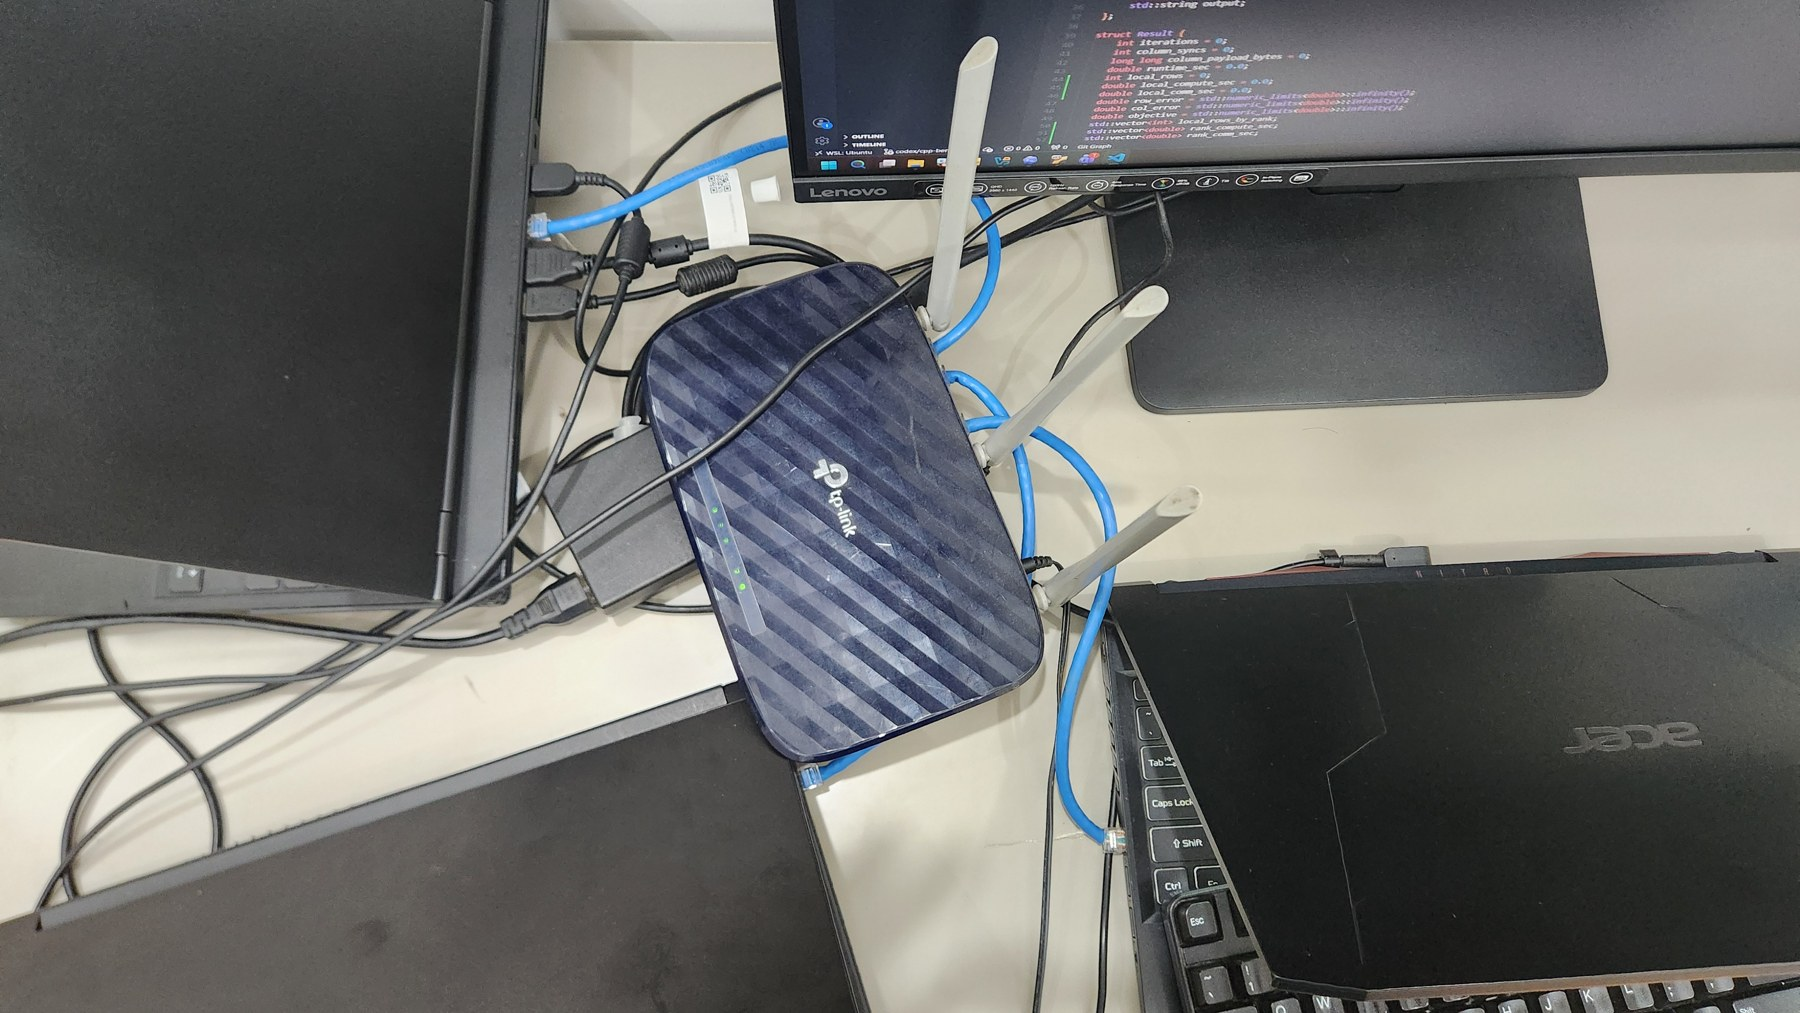
\includegraphics[height=6.2cm,keepaspectratio]{router_cluster_photo.jpg}%
}{%
\IfFileExists{assets/router_cluster_photo.png}{%
  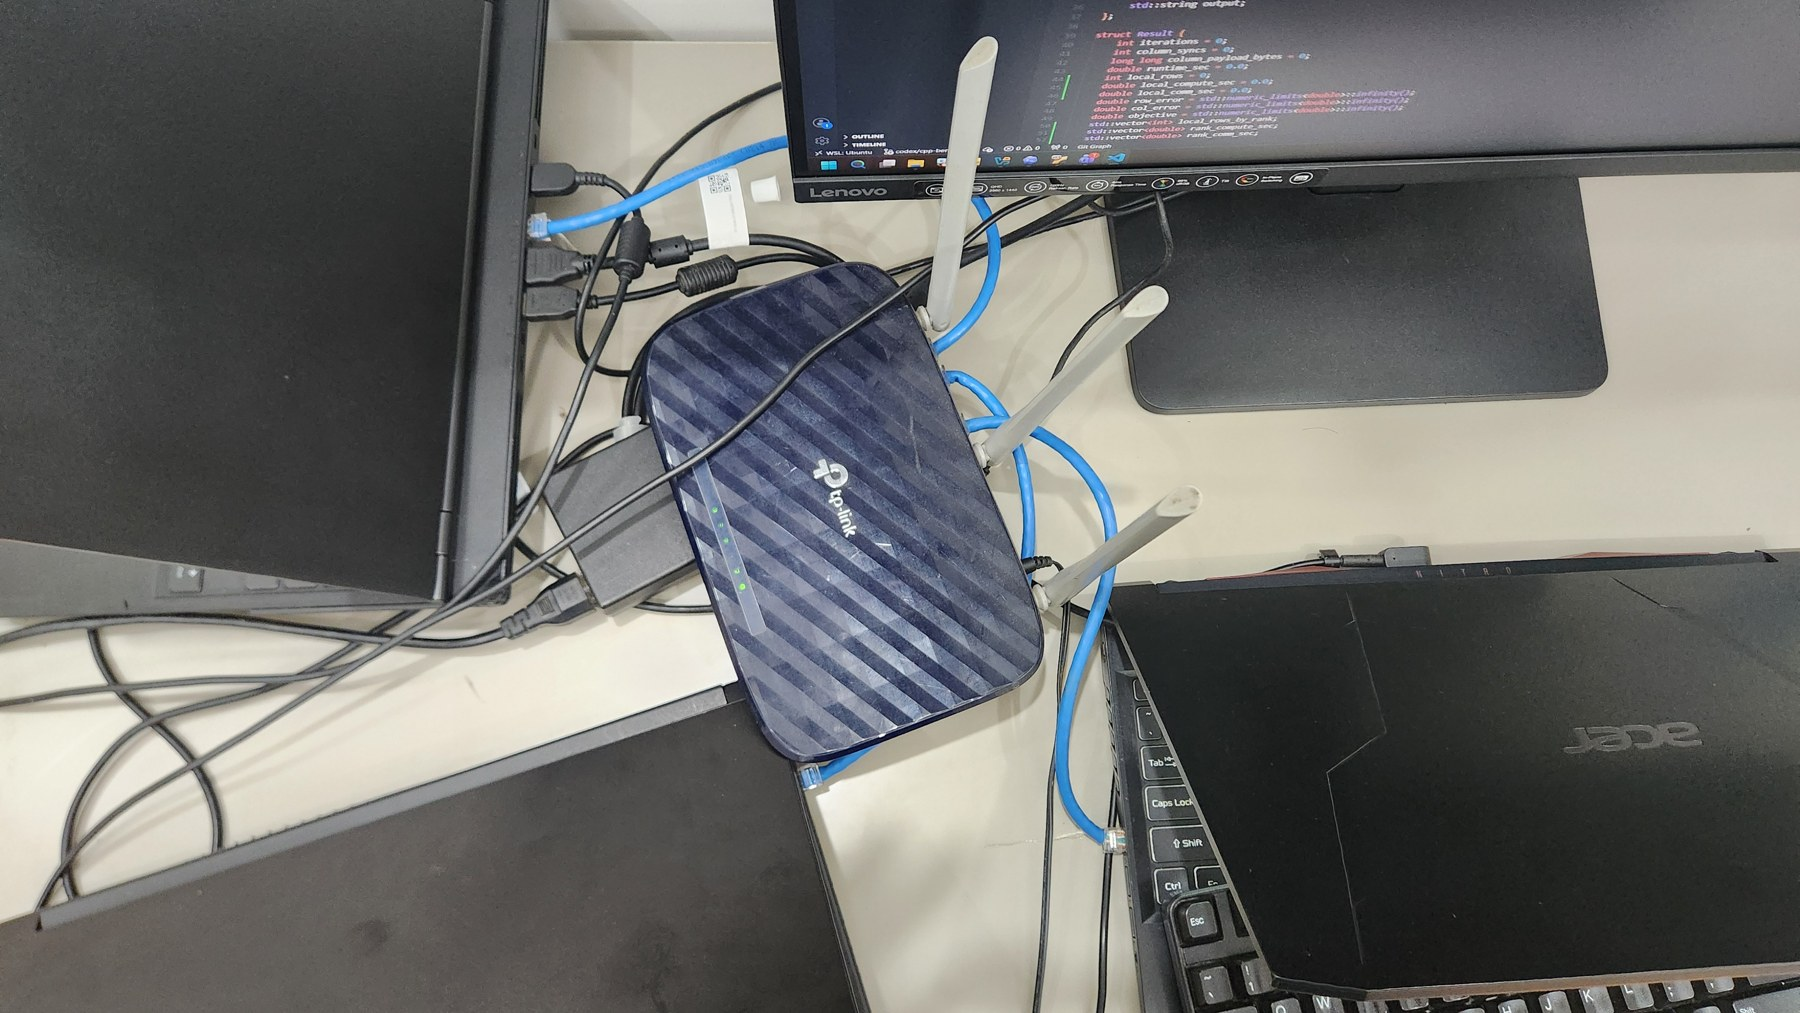
\includegraphics[height=6.2cm,keepaspectratio]{router_cluster_photo.png}%
}{%
  \fbox{\begin{minipage}[c][4cm][c]{0.86\linewidth}
  \centering
  Placeholder for the physical evidence photo.\\[0.2cm]
  Insert a photo named \texttt{assets/router\_cluster\_photo.jpg} or \texttt{assets/router\_cluster\_photo.png}\\
  showing the three laptops/PCs connected through one router.
  \end{minipage}}
}}
\caption{Three physical machines connected through one router for the MPI cluster.}
\end{figure}

\subsection{Router Setup Procedure}

The router setup used static IPv4 addresses to avoid SSH and MPI host discovery changing between runs. On each Ubuntu VM, the network interface was checked with:

\begin{verbatim}
ip -br addr
ip route
\end{verbatim}

When NetworkManager was unavailable, static addressing was configured through Netplan. A typical master configuration was:

\begin{verbatim}
network:
  version: 2
  renderer: networkd
  ethernets:
    enp0s3:
      dhcp4: no
      addresses: [192.168.1.25/24]
      routes:
        - to: default
          via: 192.168.1.1
      nameservers:
        addresses: [8.8.8.8, 1.1.1.1]
\end{verbatim}

The workers used the same subnet with different addresses, for example \texttt{192.168.1.26/24} and \texttt{192.168.1.75/24}. After applying Netplan, connectivity was validated with \texttt{ping} and \texttt{ssh}.

\subsection{MPI Hostfile and Smoke Test}

For the stable router baseline, the hostfile was:

\begin{verbatim}
192.168.1.25 slots=2
192.168.1.26 slots=2
192.168.1.75 slots=2
\end{verbatim}

The basic MPI smoke test was:

\begin{verbatim}
mpirun -np 3 --hostfile hosts_router_3_slots2 \
  --map-by node \
  --mca btl tcp,self \
  --mca btl_tcp_if_include enp0s3 \
  --mca oob_tcp_if_include enp0s3 \
  hostname
\end{verbatim}

The same pattern was used for benchmarks, replacing \texttt{hostname} with \texttt{sinkhorn\_cpp --mode mpi ...}.

\section{Correctness Validation}

Correctness was validated by running sequential and MPI modes with the same $N$, seed, $\varepsilon$, cost mode, and iteration count. The MPI result is accepted if objective and marginal errors match the sequential run within floating-point tolerance.

Across the Wi-Fi three-node sweep, the maximum objective difference remains at floating-point scale. For example, at $N=12000$, the maximum objective difference is $6.448\times 10^{-14}$. This is expected because the MPI reduction changes the order of floating-point addition, but not the mathematical computation.

\section{Experimental Plan}

The experiments follow the requirements in the task file:

\begin{enumerate}
  \item \textbf{Input-size calibration}: run $N=2000..12000$ with fixed 50 iterations. Then keep $N=8000$ and increase iterations to reach a two- to three-minute workload.
  \item \textbf{Granularity/load-balance analysis}: use the calibrated long workload and plot per-rank compute/communication time.
  \item \textbf{Speedup analysis}: run the $2N=16000$ case with process counts 1, 2, 4, and 8.
  \item \textbf{Network comparison}: compare router/Ethernet, Wi-Fi, same-band Wi-Fi, and phone-hotspot experiments.
  \item \textbf{Dynamic scheduling}: compare contiguous static partitioning with weighted chunk modes and runtime queue mode.
\end{enumerate}

\section{Baseline Router and Wi-Fi Results}

\subsection{Input-Size Sweep}

\begin{figure}[H]
\centering
\begin{subfigure}{0.49\linewidth}
\centering
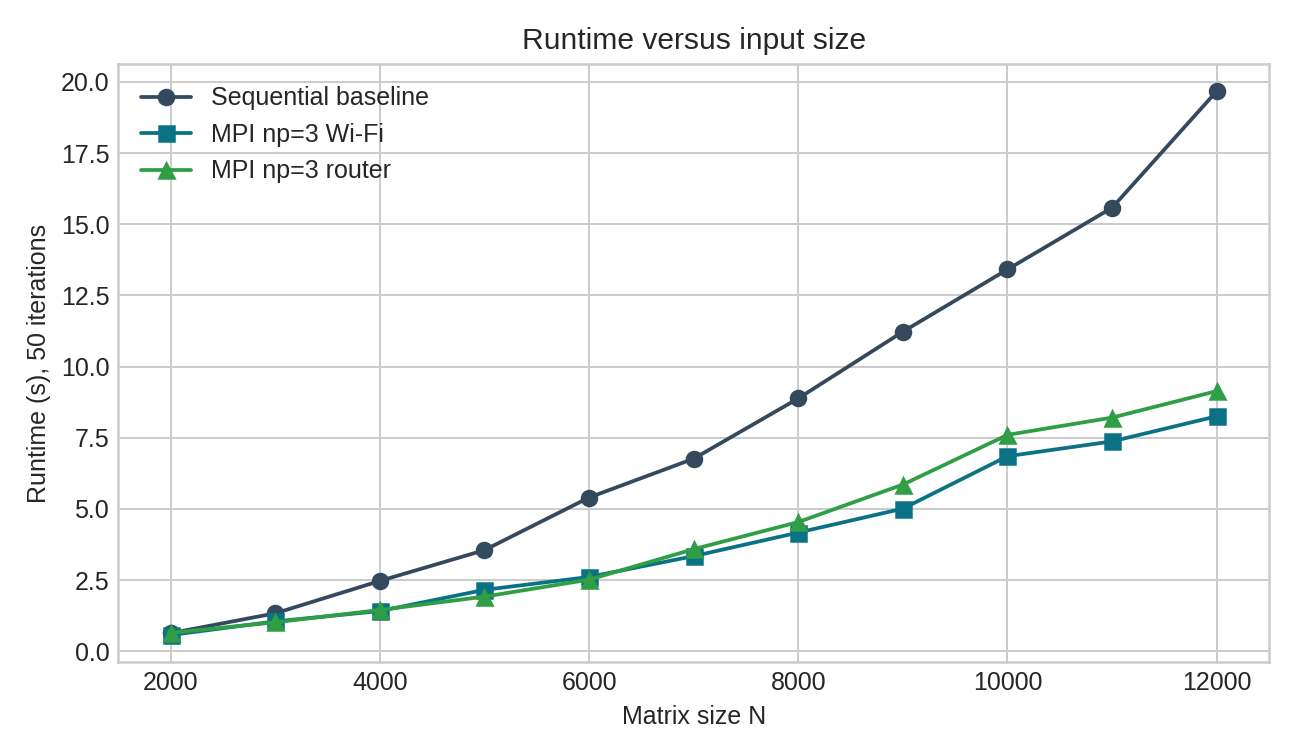
\includegraphics[width=\linewidth]{runtime_vs_size.png}
\caption{Runtime versus input size.}
\end{subfigure}
\hfill
\begin{subfigure}{0.49\linewidth}
\centering
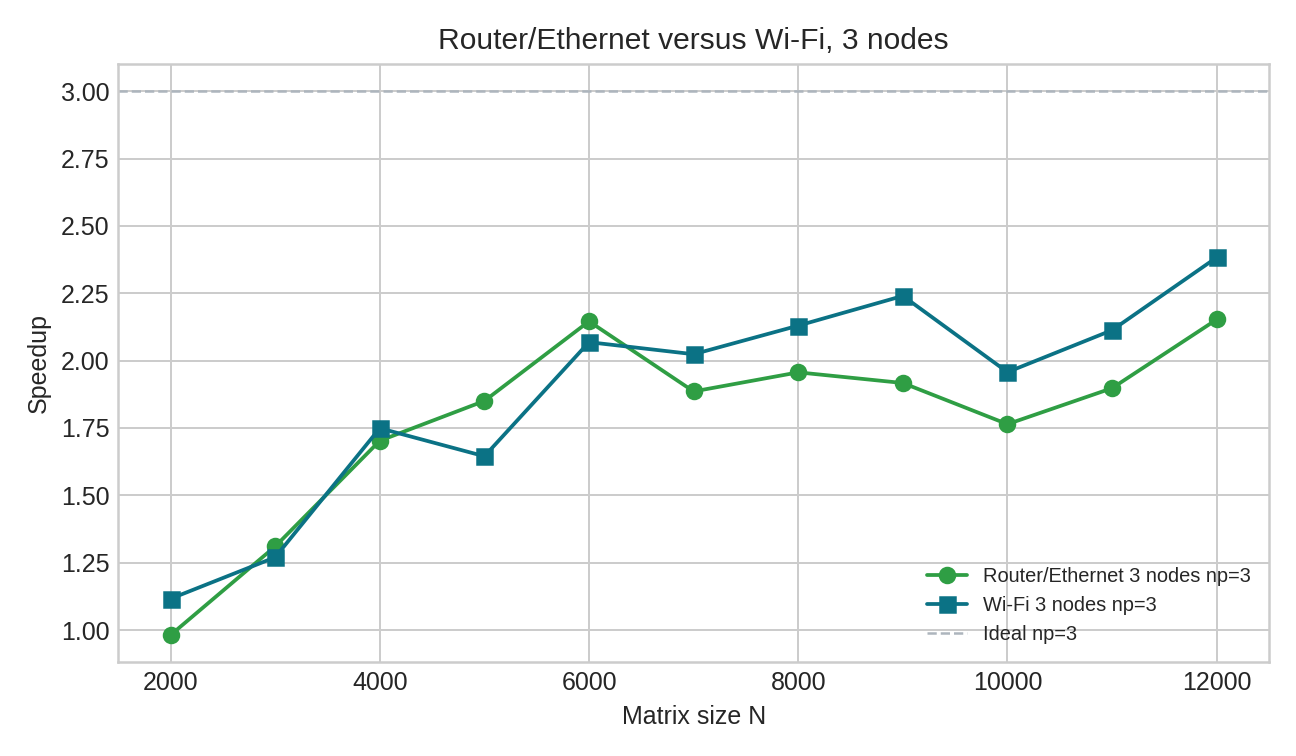
\includegraphics[width=\linewidth]{router_vs_wifi3_speedup.png}
\caption{Three-node speedup.}
\end{subfigure}
\caption{Input-size sweep and router/Ethernet versus Wi-Fi comparison with 50 Sinkhorn iterations.}
\end{figure}

\begin{table}[H]
\centering
\begin{tabular}{rrrrrr}
\toprule
$N$ & Seq avg (s) & Router np3 (s) & Router speedup & Wi-Fi np3 (s) & Wi-Fi speedup \\
\midrule
4000 & 2.471 & 1.616 & 1.529 & 1.413 & 1.749 \\
8000 & 8.881 & 3.945 & 2.251 & 4.170 & 2.130 \\
12000 & 19.673 & 8.901 & 2.210 & 8.255 & 2.383 \\
\bottomrule
\end{tabular}
\caption{Representative router/Ethernet and Wi-Fi results.}
\end{table}

The main conclusion is that MPI becomes beneficial when $N$ is large enough. Small sizes are dominated by startup, memory allocation, and communication overhead. At $N=8000$--$12000$, both router and Wi-Fi runs reach around $2.1\times$--$2.4\times$ speedup on three processes.

Router/Ethernet is more stable operationally: it avoided the intermittent Wi-Fi master disappearance observed during one Wi-Fi run. However, raw runtime does not always make router faster, because the machines are heterogeneous and VM scheduling noise is significant. Therefore, the correct conclusion is not ``router always wins'', but rather: router is a more reliable demo network, while performance still depends on node speed and run noise.

The best three-node router result observed in an earlier fixed-50 benchmark is stronger than the later safe-suite average: at $N=12000$, the run \texttt{bench\_cpp\_router3\_25\_26\_75\_fixed50\_reps4} reports 6.817 s MPI runtime, $2.8859\times$ speedup, and 0.962 efficiency. We treat this as the best observed point, while the later router/Wi-Fi report-suite results are used as the more conservative comparison set.

\subsection{Process Sweep and Efficiency}

\begin{figure}[H]
\centering
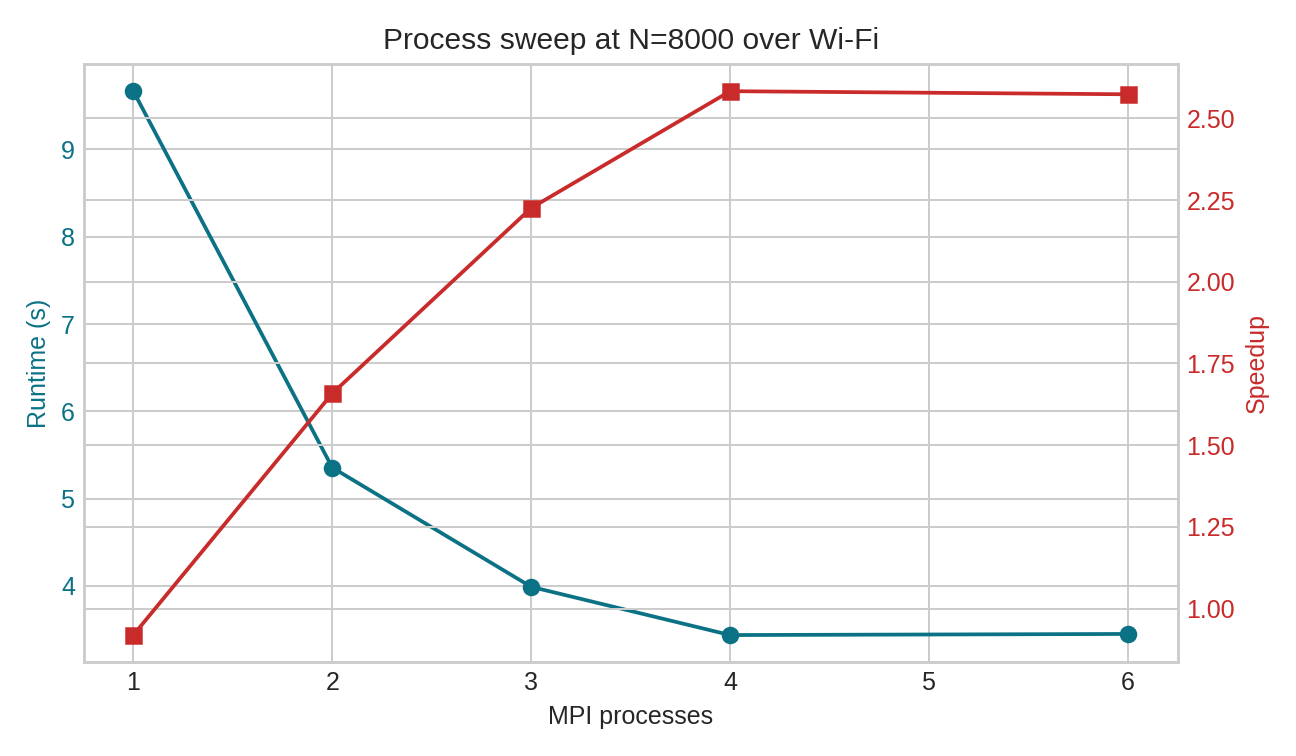
\includegraphics[width=0.91\linewidth]{process_sweep_wifi.png}
\caption{Runtime and speedup when varying process count at $N=8000$ over Wi-Fi.}
\end{figure}

\begin{table}[H]
\centering
\begin{tabular}{rrrrr}
\toprule
Processes & Runtime (s) & Speedup & Efficiency & Avg imbalance (\%) \\
\midrule
1 & 9.667 & 0.919 & 0.919 & 0.000 \\
2 & 5.355 & 1.658 & 0.829 & 0.048 \\
3 & 3.990 & 2.226 & 0.742 & 0.191 \\
4 & 3.438 & 2.583 & 0.646 & 0.512 \\
6 & 3.450 & 2.574 & 0.429 & 0.452 \\
\bottomrule
\end{tabular}
\caption{Wi-Fi process sweep at $N=8000$, 50 iterations.}
\end{table}

Runtime improves from one to four processes, but six processes do not improve over four. This is the clearest sign of communication overhead: when each rank owns fewer rows, local compute shrinks but the Allreduce vector is still length $N$ in every iteration.

\section{Required Calibration and Load-Balance Results}

\subsection{Two- to Three-Minute Workload}

\begin{figure}[H]
\centering
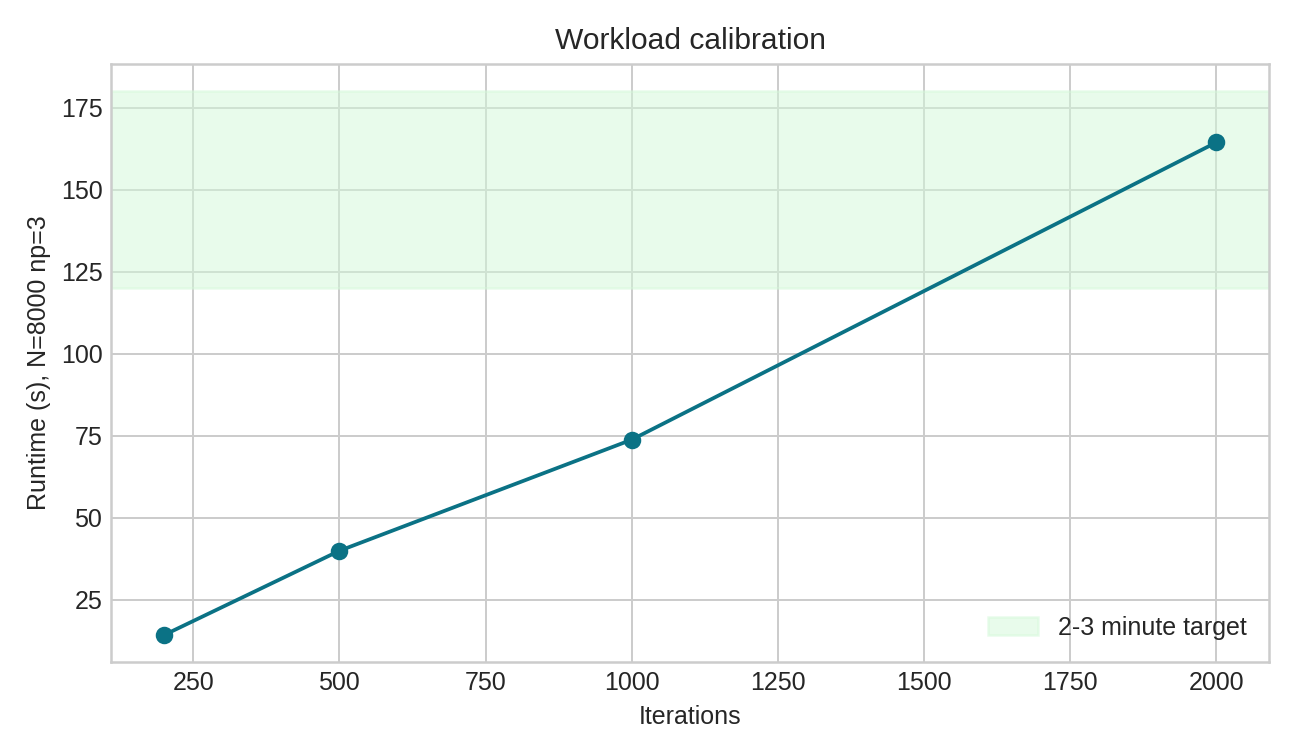
\includegraphics[width=0.91\linewidth]{workload_calibration.png}
\caption{Workload calibration at $N=8000$, \texttt{np=3}.}
\end{figure}

\begin{table}[H]
\centering
\begin{tabular}{rrl}
\toprule
Iterations & Runtime (s) & Interpretation \\
\midrule
200 & 14.176 & Too short \\
500 & 39.864 & Below one minute \\
1000 & 73.746 & Around 1.2 minutes \\
2000 & 164.394 & Within the target two- to three-minute range \\
\bottomrule
\end{tabular}
\caption{Long workload calibration.}
\end{table}

The task asks for an input size/workload whose full runtime is about two to three minutes. Increasing $N$ too far would push the dense matrix into high RAM pressure, so the safer calibration is $N=8000$ with 2000 iterations. This reaches 164.394 seconds and is used for the load-balance analysis.

\subsection{Per-Rank Load Balance}

\begin{figure}[H]
\centering
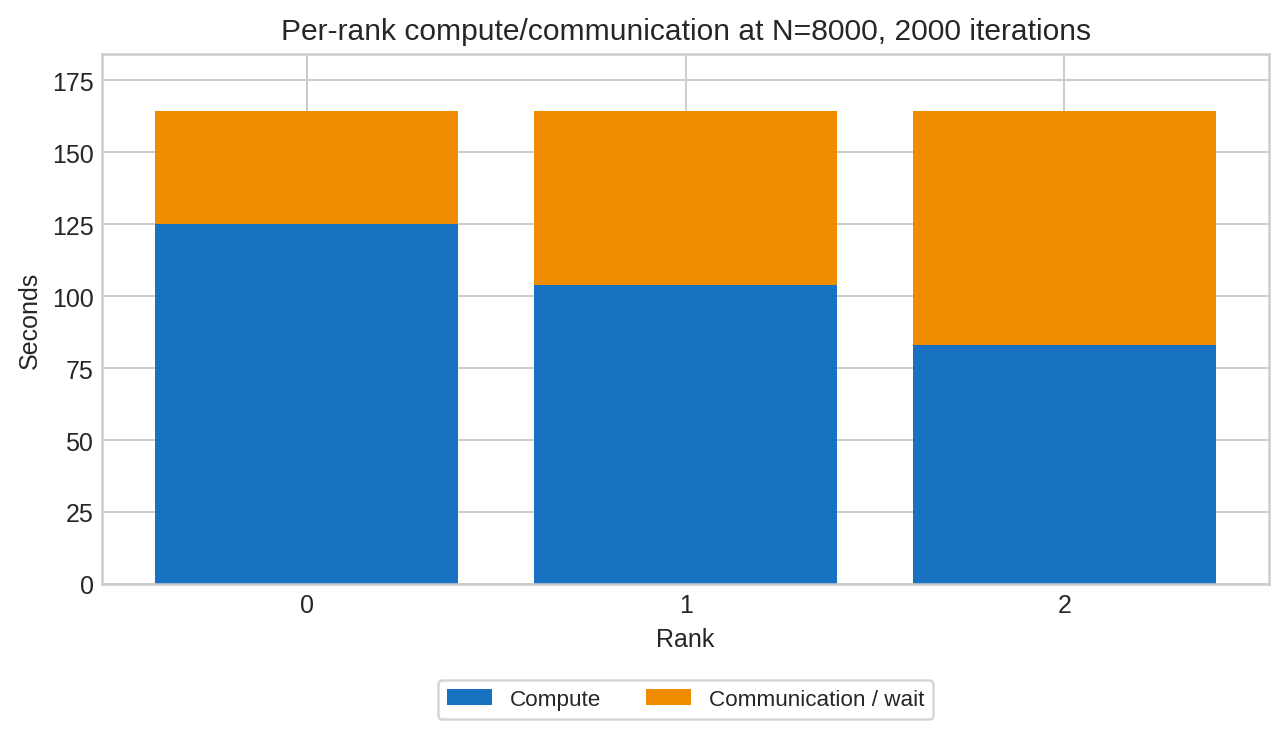
\includegraphics[width=0.91\linewidth]{load_balance_stacked.png}
\caption{Per-rank compute and communication time on the long workload.}
\end{figure}

\begin{table}[H]
\centering
\begin{tabular}{rrrrr}
\toprule
Rank & Local rows & Total (s) & Compute (s) & Communication/wait (s) \\
\midrule
0 & 2667 & 164.390 & 125.182 & 39.189 \\
1 & 2667 & 164.394 & 103.973 & 60.406 \\
2 & 2666 & 164.393 & 83.085 & 81.283 \\
\bottomrule
\end{tabular}
\caption{Per-rank breakdown at $N=8000$, 2000 iterations, \texttt{np=3}.}
\end{table}

Total time is almost identical because all ranks synchronize at the collective operation. The compute/communication split reveals heterogeneity: rank 0 computes more and waits less, while rank 2 computes less and waits more. Since total runtime difference is far below 25\%, the static contiguous partition satisfies the assignment's load-balance requirement. Still, this is exactly why dynamic weighted scheduling is worth testing: faster ranks can be assigned more rows.

\section{Speedup at the $2N=16000$ Input}

\begin{figure}[H]
\centering
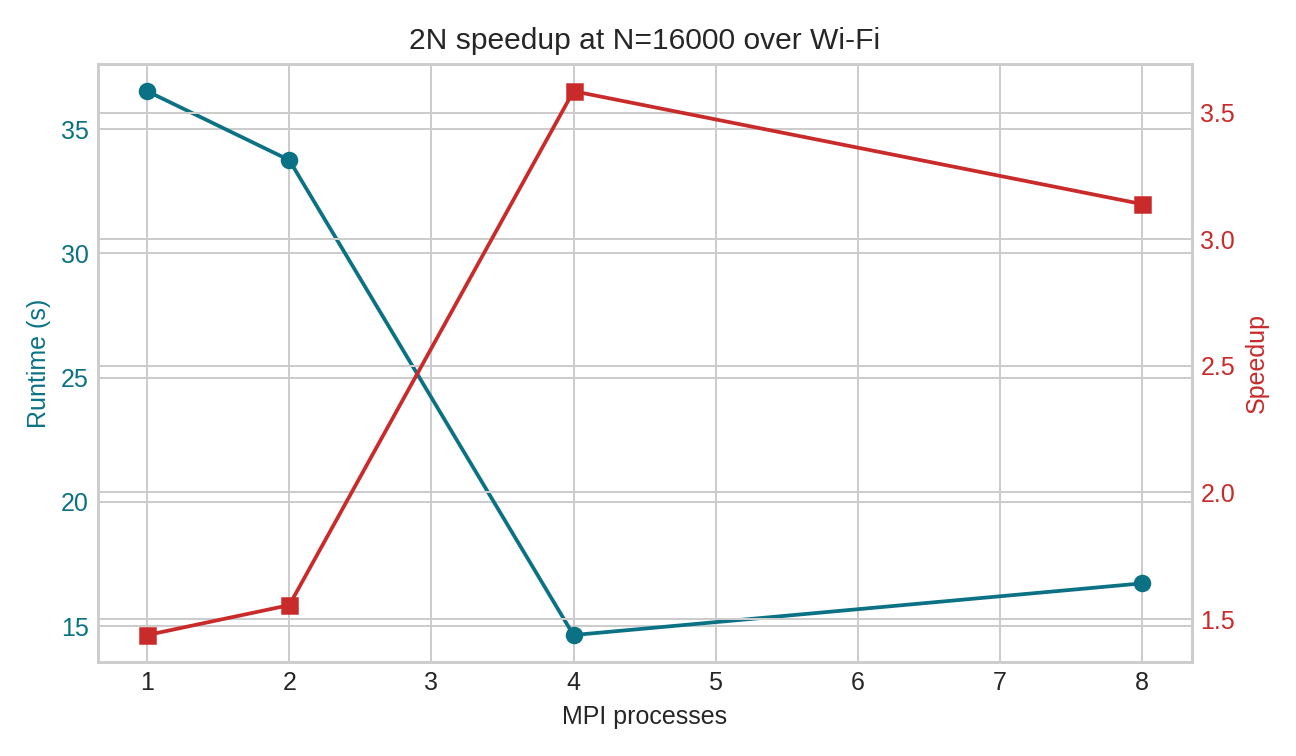
\includegraphics[width=0.91\linewidth]{speedup_2n_wifi.png}
\caption{Speedup analysis at $N=16000$ over Wi-Fi.}
\end{figure}

\begin{table}[H]
\centering
\begin{tabular}{rrrr}
\toprule
Processes & Runtime (s) & Speedup & Efficiency \\
\midrule
1 & 36.525 & 1.437 & 1.437 \\
2 & 33.750 & 1.555 & 0.778 \\
4 & 14.642 & 3.585 & 0.896 \\
8 & 16.721 & 3.139 & 0.392 \\
\bottomrule
\end{tabular}
\caption{Speedup at $N=16000$, 50 iterations.}
\end{table}

The best result is \texttt{np=4}, which reaches $3.585\times$ speedup. Increasing to \texttt{np=8} makes the run slower. This confirms the communication bottleneck: beyond a certain process count, the reduction of a length-$N$ column vector costs more than the saved local compute.

\section{Short Python Prototype Comparison}

The project started with a Python/mpi4py MVP because it was faster to validate the mathematical algorithm and correctness checks. This prototype is not the main implementation. The final benchmark path uses C++/MPI because the assignment requires C/C++, and because C++ gives direct control over memory layout, per-rank timing, communication modes, and dynamic partitioning.

\begin{figure}[H]
\centering
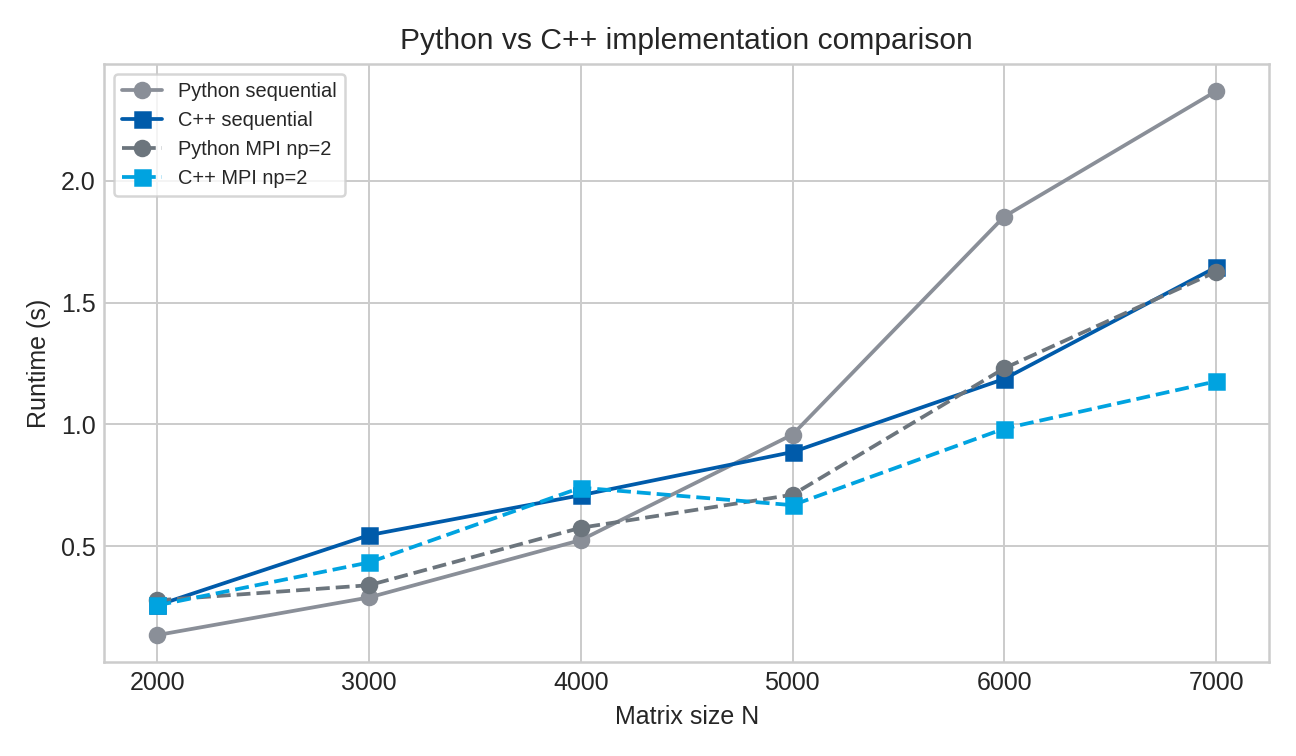
\includegraphics[width=0.76\linewidth]{python_vs_cpp.png}
\caption{Python prototype versus C++ implementation on a two-node benchmark, 3-run averages.}
\end{figure}

The result is mixed at very small sizes because fixed overhead and implementation differences dominate. From $N=5000$ onward in this two-node benchmark, the C++ MPI implementation becomes faster than the Python MPI prototype. Therefore, Python is kept only as a short validation and development reference; the analysis sections focus on the C++ solver.

\section{Network and Wireless-Band Experiments}

\subsection{Two-Node Same-Band Wi-Fi versus Phone Hotspot}

Before the three-machine router setup, the project also tested two-node Wi-Fi configurations. The same-band Wi-Fi benchmark used two VMs on the same Wi-Fi band with \texttt{np=2}. A phone-hotspot benchmark used two VMs through a different access link and was run for smaller sizes.

\begin{figure}[H]
\centering
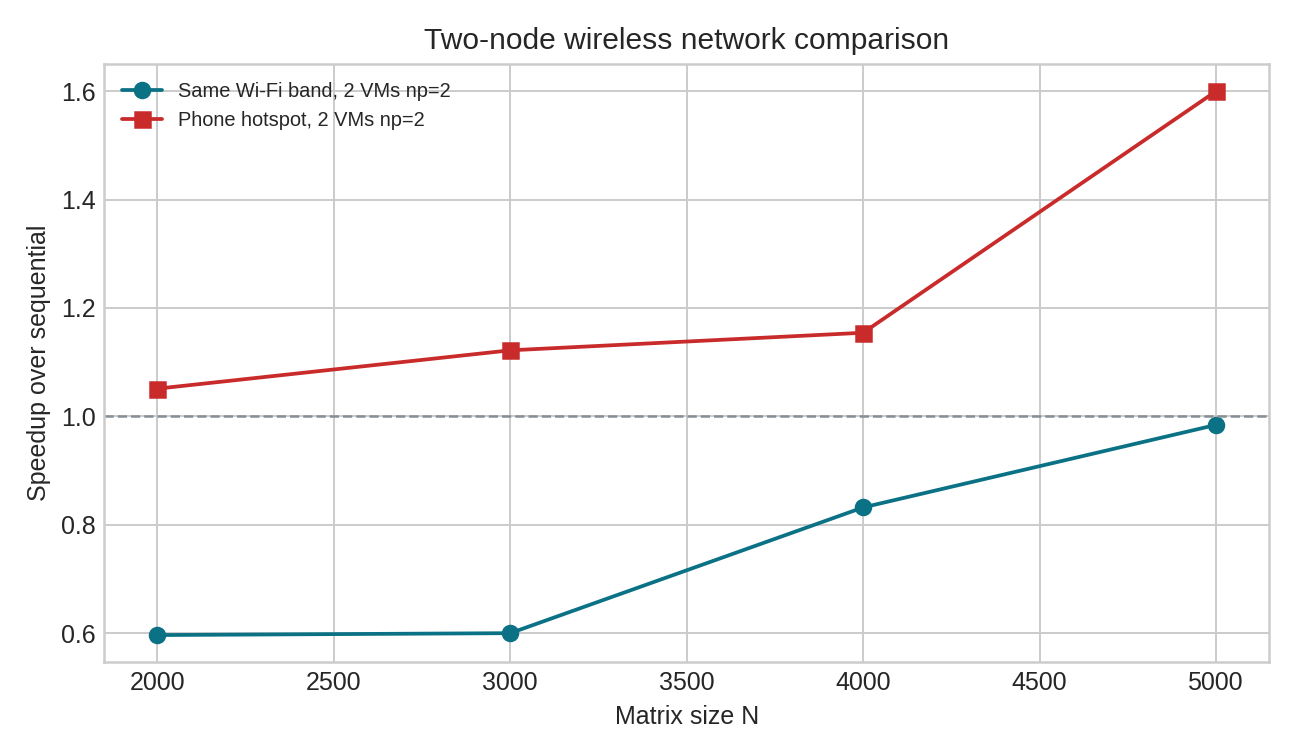
\includegraphics[width=0.91\linewidth]{network_2node_comparison.png}
\caption{Two-node wireless topology comparison on overlapping sizes.}
\end{figure}

\begin{table}[H]
\centering
\begin{tabular}{rrrrr}
\toprule
$N$ & Same-band speedup & Same-band MPI (s) & Hotspot speedup & Hotspot MPI (s) \\
\midrule
2000 & 0.596 & 0.824 & 1.051 & 0.681 \\
3000 & 0.600 & 1.531 & 1.122 & 1.269 \\
4000 & 0.832 & 2.010 & 1.154 & 2.192 \\
5000 & 0.984 & 2.601 & 1.600 & 2.639 \\
\bottomrule
\end{tabular}
\caption{Same-band Wi-Fi and phone-hotspot comparison for two-node runs.}
\end{table}

The conclusion is subtle. Same-band Wi-Fi had low ping before the benchmark, but MPI did not outperform sequential until around $N=6000$. The phone-hotspot run showed better speedup for $N=2000$--$5000$, but it used a smaller test range and a different access link. Therefore, it should be treated as evidence that wireless topology matters, not as a universal claim that hotspot is better. A strict same-router same-band versus different-band comparison should be added if a controlled dual-band router experiment is run later.

\subsection{Communication-Reduction Variants}

The same-band Wi-Fi setup was also used to test communication variants. These do not change the router setup, but they answer an important question: since Allreduce is the bottleneck, does reducing column synchronization payload improve performance?

\begin{figure}[H]
\centering
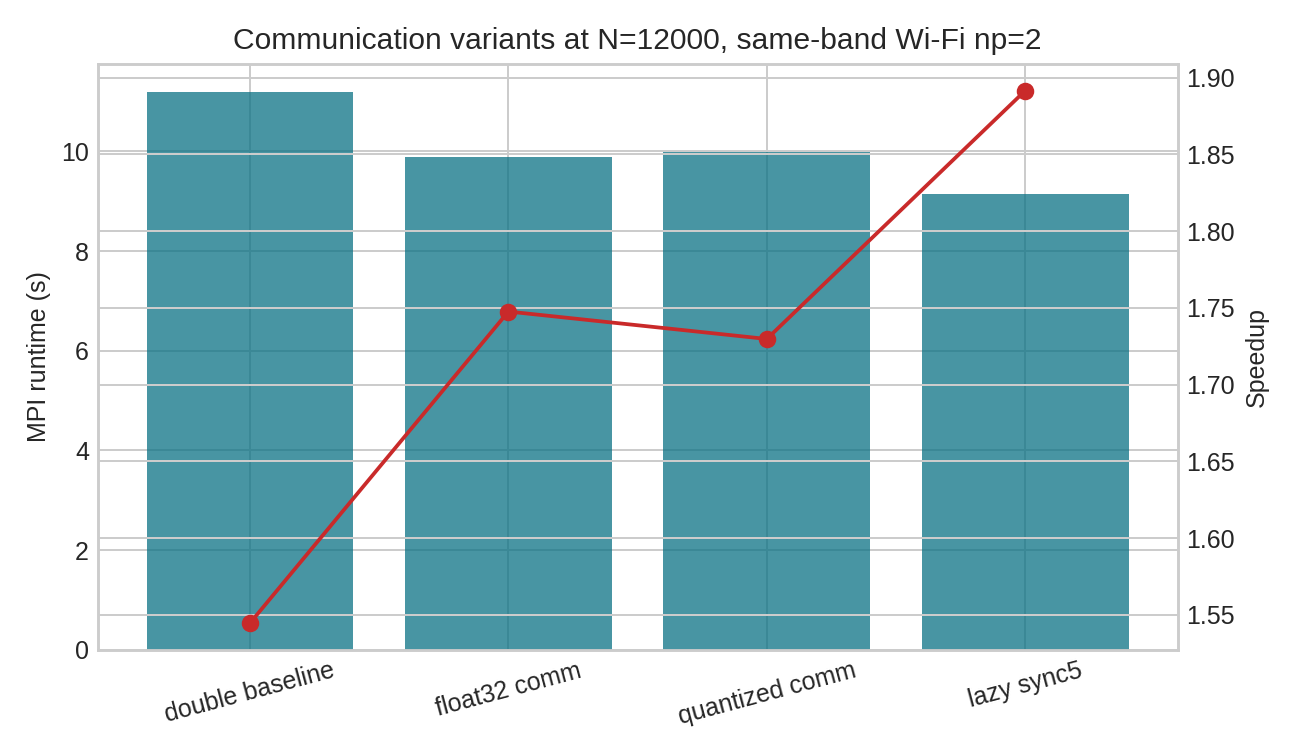
\includegraphics[width=0.91\linewidth]{comm_variants_12000.png}
\caption{Communication variants at $N=12000$, same-band Wi-Fi, \texttt{np=2}.}
\end{figure}

\begin{table}[H]
\centering
\begin{tabular}{lrrr}
\toprule
Variant & Payload ratio & MPI runtime (s) & Speedup \\
\midrule
Double baseline & 1.0 & 11.196 & 1.545 \\
Float32 communication & 0.5 & 9.895 & 1.748 \\
Quantized communication & 0.5 & 9.997 & 1.730 \\
Lazy sync every 5 iterations & 0.2 & 9.142 & 1.892 \\
\bottomrule
\end{tabular}
\caption{Communication variant results at $N=12000$.}
\end{table}

Lazy synchronization gives the strongest speedup because it reduces the main column synchronization frequency to 20\% of the baseline. Float32 communication is a safer compression-style optimization: it halves payload and improves runtime, with small objective differences around $10^{-10}$--$10^{-11}$. Quantization also halves payload but adds packing overhead and larger numerical error.

\section{Four-Machine Wi-Fi Experiment}

An earlier four-machine Wi-Fi run used \texttt{np=4} on hosts \texttt{192.168.1.105}, \texttt{192.168.1.227}, \texttt{192.168.1.159}, and \texttt{192.168.1.190}. The run completed all 88 expected JSON files for sizes $2000$--$12000$ and four repetitions.

\begin{table}[H]
\centering
\begin{tabular}{rrrr}
\toprule
$N$ & Seq avg (s) & MPI np4 avg (s) & Speedup \\
\midrule
4000 & 2.471 & 1.528 & 1.617 \\
8000 & 8.881 & 3.451 & 2.574 \\
10000 & 13.411 & 4.660 & 2.878 \\
12000 & 19.673 & 6.143 & 3.203 \\
\bottomrule
\end{tabular}
\caption{Four-machine Wi-Fi representative results.}
\end{table}

This shows that adding a fourth machine can help for large $N$: at $N=12000$, the speedup is about $3.20\times$. However, the later controlled router/Wi-Fi experiments focused on three machines because the four-machine Wi-Fi cluster was harder to keep stable after node/IP changes.

\section{Dynamic Scheduling Experiments}

\subsection{Implemented Dynamic Modes}

The dynamic branch extends the static row partition with chunk-based modes:

\begin{itemize}
  \item \textbf{contiguous}: original static contiguous row ownership.
  \item \textbf{weighted-chunk equal}: split rows into chunks but use equal rank weights.
  \item \textbf{weighted-chunk adaptive}: use rank throughput from previous repetitions to suggest weights.
  \item \textbf{weighted manual 2,1,1}: manually assign more work to rank 0.
  \item \textbf{runtime queue}: experimental queue-based chunk assignment, tested only at small sizes due to overhead.
\end{itemize}

\subsection{Does Dynamic Scheduling Improve Performance?}

\begin{figure}[H]
\centering
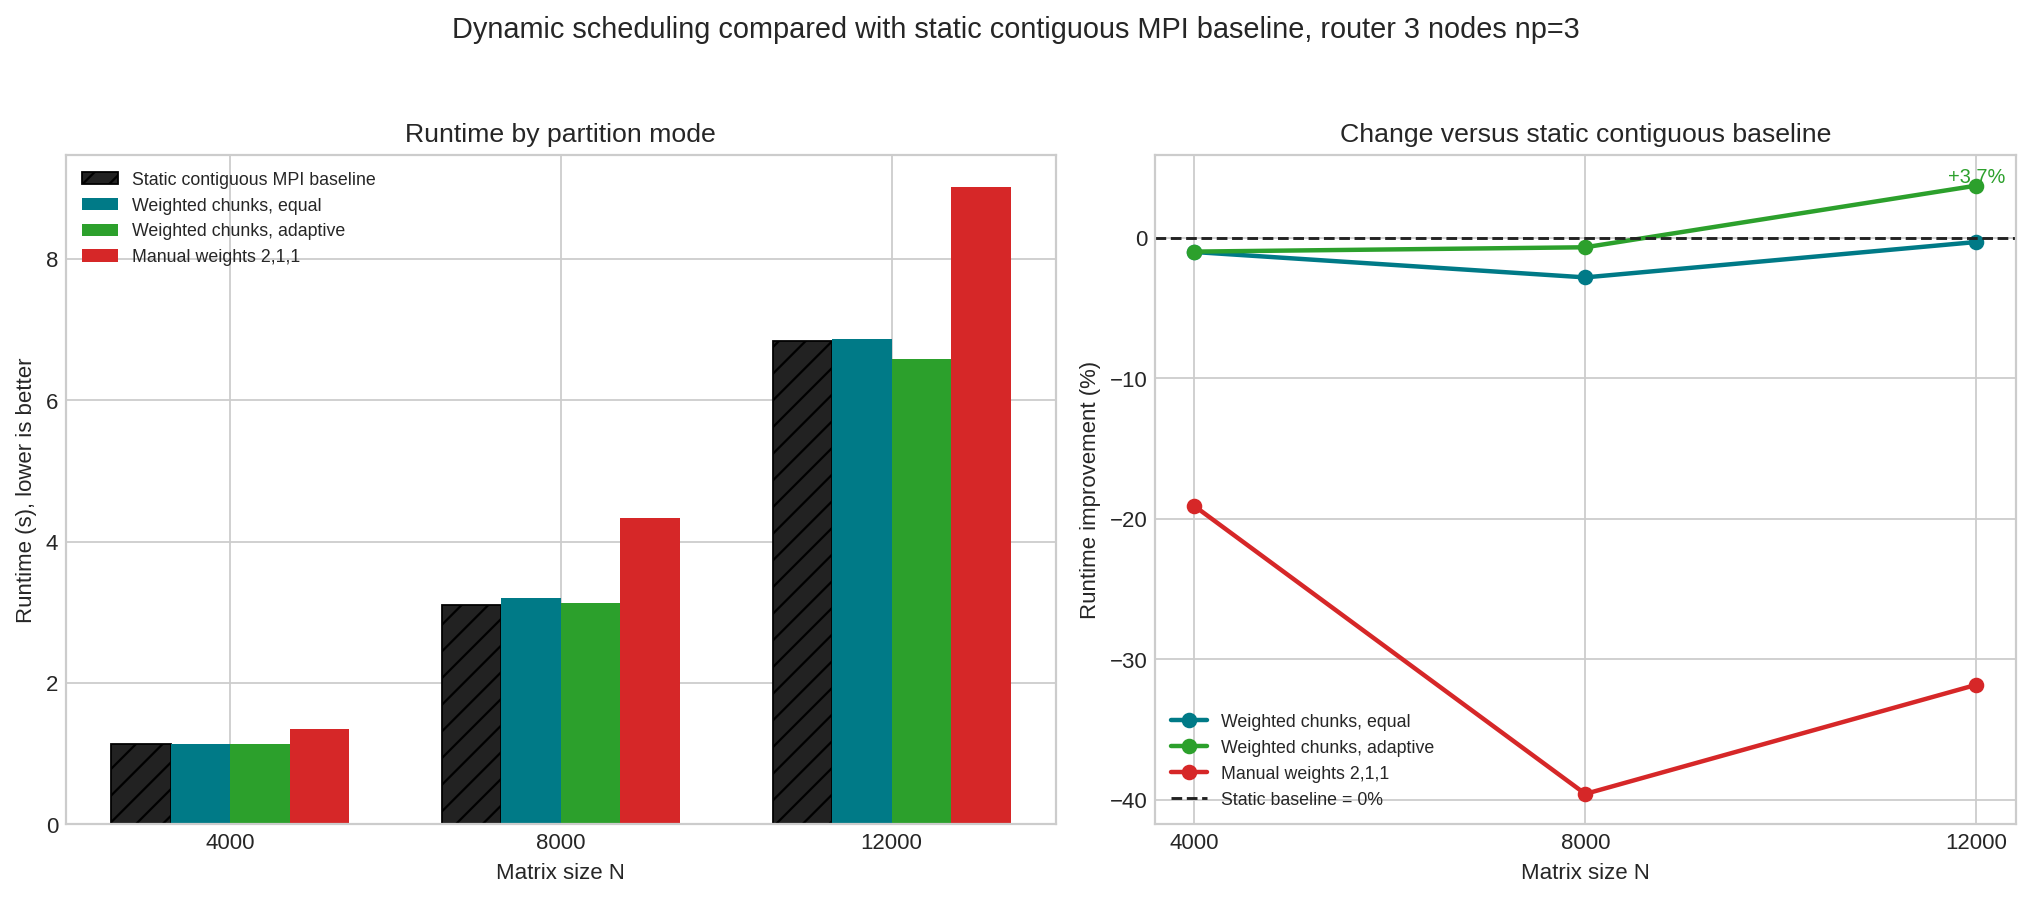
\includegraphics[width=0.91\linewidth]{dynamic_modes_np3.png}
\caption{Dynamic partition modes on router 3 nodes, \texttt{np=3}. The static contiguous MPI partition is the baseline; it is already distributed across machines but assigns one fixed row interval to each rank.}
\end{figure}

\begin{table}[H]
\centering
\begin{tabular}{rrrrr}
\toprule
$N$ & Static contiguous MPI (s) & Weighted equal (s) & Adaptive (s) & Best result \\
\midrule
4000 & 1.129 & 1.141 & 1.140 & Contiguous \\
8000 & 3.108 & 3.195 & 3.128 & Contiguous \\
10000 & 4.725 & 4.737 & 4.644 & Adaptive by 1.7\% \\
12000 & 6.839 & 6.858 & 6.584 & Adaptive by 3.7\% \\
\bottomrule
\end{tabular}
\caption{Dynamic scheduling summary on router 3 nodes, \texttt{np=3}.}
\end{table}

Dynamic scheduling is not a universal improvement. At smaller sizes, chunk overhead and less cache-friendly ownership can cancel the benefit. At larger sizes, adaptive weights begin to help: at $N=12000$, adaptive weighted chunks improve runtime by about 3.7\% over contiguous.

\begin{figure}[H]
\centering
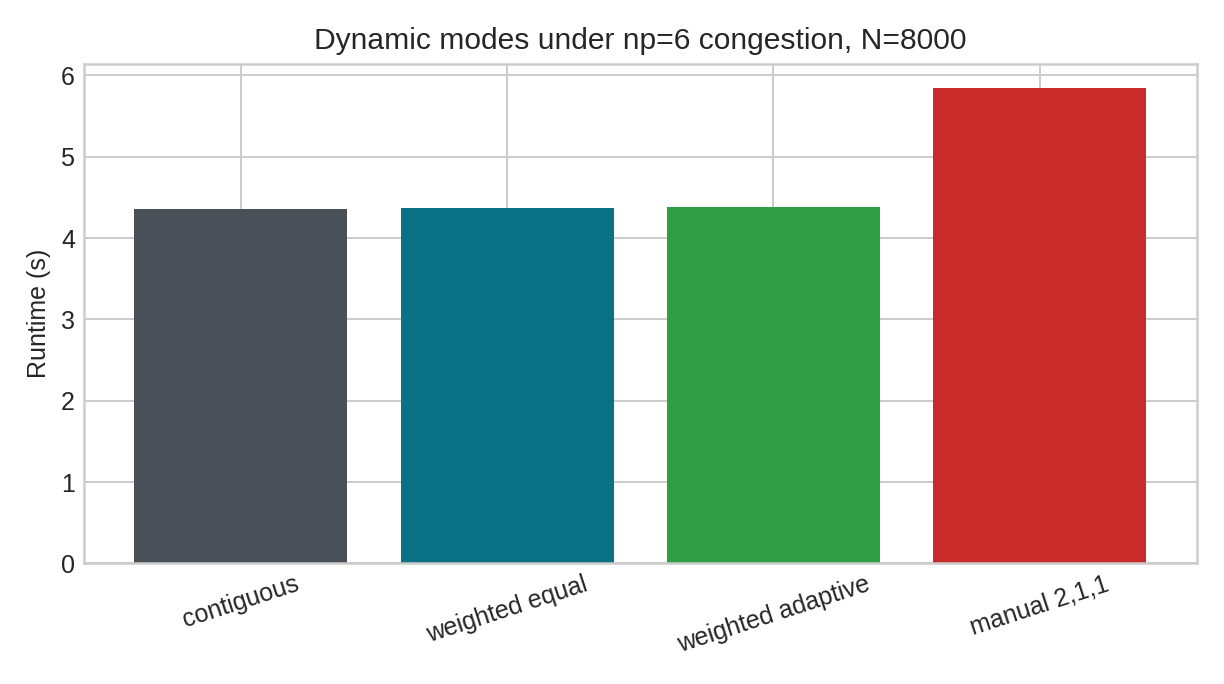
\includegraphics[width=0.86\linewidth]{dynamic_np6_congestion.png}
\caption{Dynamic modes under \texttt{np=6} congestion at $N=8000$.}
\end{figure}

Under the more congested \texttt{np=6} setting at $N=8000$, contiguous, weighted-equal, and weighted-adaptive are very close: 4.354 s, 4.367 s, and 4.382 s respectively. Manual \texttt{2,1,1} is much worse at 5.848 s because it over-assigns work to one rank. Runtime queue is correct as an experiment but far slower at small sizes: for example, around 2.18 s versus 0.58 s at $N=2000$, and around 6.04 s versus 1.13 s at $N=4000$. Therefore, the practical dynamic result is:

\begin{itemize}
  \item Adaptive weighted chunks can improve large balanced runs slightly.
  \item Manual weights can hurt badly if the assumption about machine speed is wrong.
  \item Runtime queue is useful to demonstrate dynamic assignment but not suitable as the performance path in this implementation.
\end{itemize}

\section{Discussion}

\subsection{What the Experiments Show}

The experiments lead to four main conclusions.

First, the Sinkhorn solver has enough computation to benefit from MPI, but only after $N$ is sufficiently large. Small runs are dominated by startup and communication overhead. Large runs at $N=8000$--$12000$ show clear speedup.

Second, the main scalability limiter is communication. The $2N=16000$ process sweep peaks at \texttt{np=4}; \texttt{np=8} is slower even though it has more processes. Communication-reduction variants support the same conclusion: reducing column synchronization payload/frequency improves runtime.

Third, router/Ethernet is the better demo setup because it is operationally more stable than Wi-Fi. Wi-Fi can still produce competitive runtimes, but it is more sensitive to route loss, band/access-point behavior, and VM host variability.

Fourth, dynamic scheduling is promising but not automatically better. The best adaptive result improves the large $N=12000$ run by about 3.7\%, but static contiguous remains excellent for many cases. Dynamic scheduling should be presented as an extension for heterogeneous clusters, not as a guaranteed replacement for static partitioning.

\subsection{Limitations}

\begin{itemize}
  \item Dense matrix storage limits safe input size because memory grows as $O(N^2)$.
  \item Wi-Fi and VM scheduling introduce noise; repeated runs are necessary.
  \item The current dynamic runtime queue recomputes/dispatches too much and is not optimized.
  \item A fully controlled same-router same-band versus different-band experiment is not yet available; current wireless evidence compares same-band Wi-Fi with a phone-hotspot access link.
\end{itemize}

\subsection{Future Work}

Future work should include a true sparse kernel representation, a 2D block decomposition for larger clusters, non-blocking collectives, and a controlled dual-band router experiment. For dynamic scheduling, the next step is to keep weighted chunks but reduce overhead and learn weights over longer runs rather than relying on short repetitions.

\section{Conclusion}

The project implements and evaluates a real C++/MPI Sinkhorn optimal transport solver on a physical-machine VM cluster. It satisfies the main course requirements: at least three physical machines, C++ source code, MPI execution, sequential validation, decomposition explanation, communication analysis, load-balance analysis, and benchmark results.

The best stable three-node MPI results reach around $2.1\times$--$2.4\times$ speedup for $N=8000$--$12000$. The four-node Wi-Fi run reaches about $3.20\times$ speedup at $N=12000$. The $2N=16000$ speedup experiment shows that \texttt{np=4} is better than \texttt{np=8}, confirming that Allreduce communication becomes the bottleneck.

The practical recommendation is to demo the project on the router/Ethernet three-machine setup, use $N=8000$ with 2000 iterations for the two- to three-minute workload, and present dynamic weighted scheduling as an advanced extension that gives small gains on large heterogeneous runs but requires careful tuning.

\end{document}
